\chapter{Realisierung}

\label{ReportRealisierung}

\section{Umsetzung}

\subsection{HTML-Prototyp}

Im Rahmen der Umsetzung wurde ein HTML-Prototyp erstellt, dieser dient als Basis
für die echte Applikation.

\begin{figure}[!htb]
  \centering
  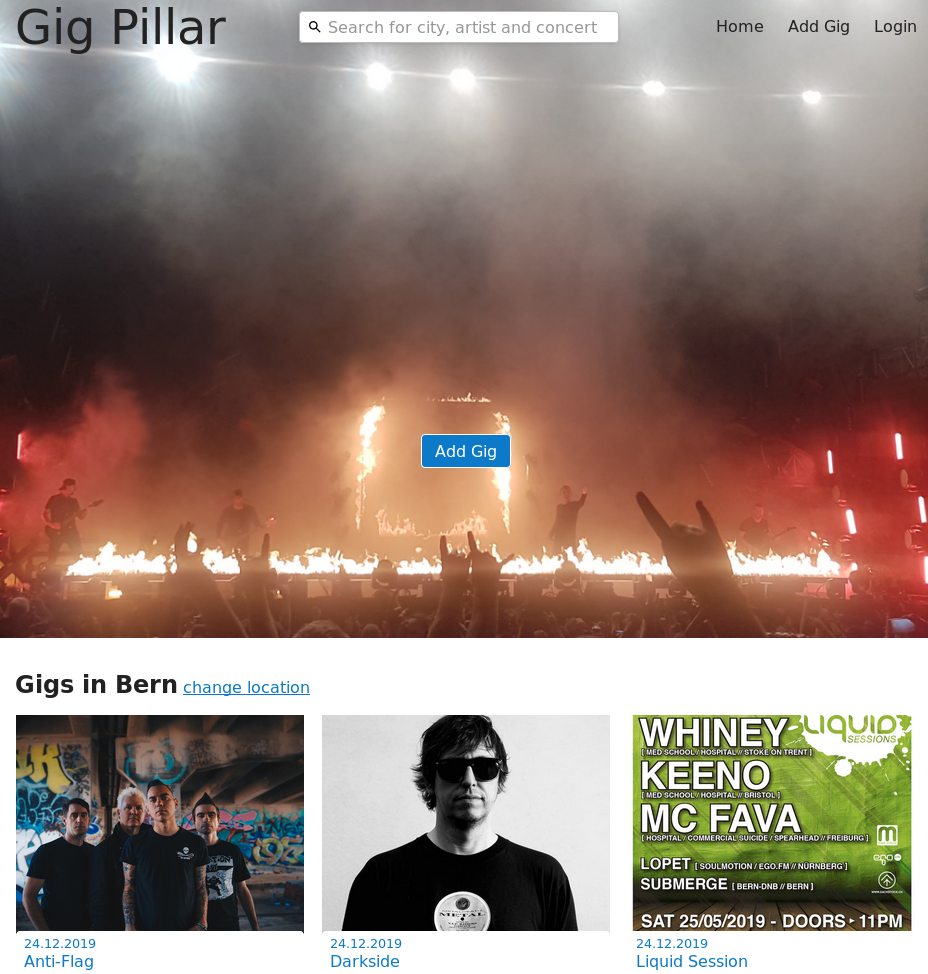
\includegraphics[width=1\textwidth]{figures/html-prototype.png}
  \caption{HTML Prototyp}
\end{figure}

\subsection{Datenbankschema}

Das finale Schema ist im Realisierungs Anhang~\ref{RealisierungsSchema}.
Folgende Änderungen wurden am von der Konzeptphase vorgegebenen Schema vorgenommen.

\subsubsection{Alle Entitäten}
Alle «created\_at» Felder wurden nach «inserted\_at» umbenannt, da dies die
Standardbenennung des Phoenix Frameworks ist.

\subsubsection{User}
Der Benutzer Entität wurde das Feld «password» nach «password\_hash» umbenannt,
damit klar ist, dass nicht ein Passwort sondern nur ein Hash abgespeichert wird.
Das Passwort wird mit \textbf{Argon2}\footnote{\url{https://en.wikipedia.org/wiki/Argon2}}
verschlüsselt und ist somit eine sichere Verschlüsselung.

\subsubsection{Genre}
Der Genre Entität sind im Konzept die Datumsfelder «update\_at» und «inserted\_at»
vergessen gegangen und wurden in der Realisierung nachgeführt.

\subsubsection{Gig}\label{RealisierungSchemaGig}
In der Gig Entität wurden drei weitere Felder hinzugefügt.
Die Felder «uuid» und «picture» dienen dazu, die beim Erfassen sowie
Bearbeiten eines Gigs hochgeladenen Bilder zu identifizieren.
Das zusätzliche Feld «tickets» ermöglicht es, beim Erfassen eines Gigs
einen Link zum Ticketvorverkauf zu hinterlegen.

\subsubsection{Location}
Die Location Entität erhielt bei der Realisierung zwei neue Felder,
«address» für die Adresse der Location und
«google\_place\_id» um die Referenz der Google API zu erhalten.

\section{Tests}

Bis auf fünf Tests im Testprotokoll konnten alle mit einem \textbf{OK}
durchgeführt werden. Einige Features wurden aufgrund von mangelnder Zeit nicht
umgesetzt. Genauere Details sind im Test Protokoll im
Realisierungsanhang~\ref{RealisierungsTestprotokoll}.
